\chapter{Metodologia}
\label{chap:Metodo}

Neste capítulo é apresentada a metodologia de pesquisa empregada neste trabalho. Inclui os procedimentos adotados para a revisão bibliográfica, a definição do escopo, o desenvolvimento do jogo. A seguir é apresentado um diagrama na Figura \ref{Fig:all_process.png}, dando destaque às grandes fases do processo de desenvolvimento do projeto.

\begin{figure}[htbp]
	\centering
		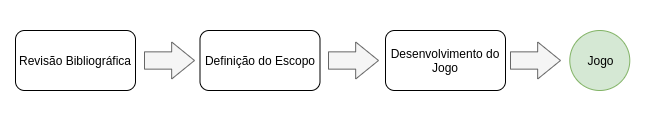
\includegraphics[keepaspectratio=true,scale=0.7]{figuras/all_process.png}
	\caption{Visão Geral do Processo Metodológico - Próprio Autor}
	\label{Fig:all_process.png}
\end{figure}

Foram adotadas algumas diretrizes e práticas da Engenharia de Software para complementar o processo de construção do jogo, buscando trazer uma maior sistemática em alguns pontos do processo \cite[p. 39]{Pressman_2000} \cite[p. 31]{Bourque_2014}. Como os princípios voltados para um Processo de Software Pessoal (PSP), por conta do jogo estar sendo desenvolvido por uma pessoa, a Engenharia de Requisitos, o processo de construção dos protótipos, a modelagem dos dados e requisitos, a definição da arquitetura do software, a especificação dos artefatos, o processo de implementação e qualidade do software \cite[p. 74]{Pressman_2000}.  % ES pg 39 / swebok xxxi; %ES pg 74


\section{Revisão Bibliográfica} 

Esta seção apresenta detalhes da primeira etapa desse trabalho, a revisão bibliográfica. Em um primeiro momento, foi realizado um estudo não sistemático dos tópicos Interação Humano-Computador, Personas e Jogos.

A busca foi realizada em livros, artigos científicos e sites eletrônicos, e a seleção dos estudos relevantes foi auxiliada pelos orientadores. A interpretação e análise crítica das informações apresentadas na literatura adotada foram feitas pelo próprio autor deste trabalho \cite{ROTHER2007}. O Capítulo \ref{chap:ref} apresenta o resultado dessa revisão bem como uma descrição de alguns trabalhos relacionados com o tema deste estudo. 

Os trabalhos correlatos foram identificado por meio de uma Revisão Sistemática de Literatura (RSL) juntamente com a técnicas de Snowballing Reveso. Detalhes sobre a metodologia usada nesta parte da pesquisa e dos resultados obtidos estão descritos no artigo de \citeonline{deSales_SousaeSilva_2020}.

Segundo \citeonline[p. 127]{Pressman_2000} essa etapa de pesquisa, revisão da literatura e análise de trabalhos semelhantes é denominada de concepção do projeto. Neste ponto do projeto é definido o entendimento básico do problema, as partes envolvidas e demais elementos que os caracterizam. A partir desta base de conhecimento o projeto prosseguiu para a definição do escopo.

\section{Definição do Escopo}

Essa fase tem como objetivo definir o público-alvo do jogo e identificar os requisitos que atendam aos objetivos destes jogadores. A elaboração e execução da coleta de dados utilizou-se de princípios de uma metodologia de pesquisa chamada survey. 

De acordo com \citeonline{Kasunic_2005} um \textit{Survey} envolve a coleta e análise de dados na qual os entrevistados respondem a um instrumento de pesquisa previamente planejado. O survey consiste na execução de sete principais atividades:

\begin{enumerate}
    \item Identificar os objetivos da pesquisa;
    \item Identificar e caracterizar o público-alvo;
    \item Elaborar o plano de amostragem;
    \item Elaborar e escrever o questionário;
    \item Aplicar teste piloto do questionário;
    \item Distribuir o questionário; e
    \item Analisar os resultados e escrever um relatório.
\end{enumerate}

O questionário tem o objetivo de identificar as características dos público-alvo e realizar o levantamento de requisitos \cite[p. 128]{Pressman_2000}. Na sequência foram definidas as personas do projeto, pois de acordo com o processo descrito em \citeauthor{usability2020} a etapa que antecede a construção das personas é a coleta de dados sobre o público-alvo. \citeonline[97,98]{cooper07} define esse processo pelas seguintes etapas:

\begin{enumerate}
    \item Identificar as variáveis comportamentais;
    \item Mapear os sujeitos da entrevista com as variáveis comportamentais;
    \item Identificar padrões de comportamento significativos;
    \item Sintetizar características e objetivos relevantes;
    \item Verificar se há redundância e integridade;
    \item Expandir a descrição de atributos e comportamentos; e
    \item Designar tipos de persona.
\end{enumerate}

Um vez definidas, as personas podem ser utilizadas em várias fases do processo. Elas servem tanto para o alinhamento de informações entre as partes envolvidas, quanto para concepção de ideias, validação do projeto e tomada de decisão \cite[p. 80]{Vianna_2014}. %design things pg 80

\section{Processo de Desenvolvimento do Jogo}

A partir dos dados obtidos na Revisão Bibliográfica e Questionário de Pesquisa, inicia-se o processo de desenvolvimento do jogo. Os requisitos, metas de experiência e o perfil do jogador identificados servem de base para essa etapa. Na Figura \ref{Fig:overview-process.png} é apresentada essa relação dos insumos gerados nas etapas anteriores ao processo de desenvolvimento do jogo.

\begin{figure}[htbp]
	\centering
		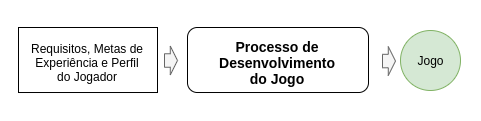
\includegraphics[keepaspectratio=true,scale=0.65]{figuras/overview-process.png}
	\caption{Relação entre Insumos e Processo de Desenvolvimento do Jogo - Próprio Autor}
	\label{Fig:overview-process.png}
\end{figure}

Na sequência é apresentado com mais detalhes sobre o \textit{Playcentric Design Process}, processo para o desenvolvimento de jogos digitais, no qual é especificado o ciclo base que fundamenta as etapas deste processo.

\subsection{Princípio Iterativo}

A abordagem \textit{Playcentric Design Process} concentra-se em envolver o jogador no processo de construção, desde a concepção até a conclusão. Dessa forma, é possível manter continuamente a experiência do jogador em mente, tendo como objetivo torná-la satisfatória para seus jogadores-alvo \cite[p. 10]{Fullerton_2008}. % playcentric pg 10

Segundo \citeonline[p. 10, 11]{Fullerton_2008} o primeiro passo para se incluir o jogador no processo de desenvolvimento de um jogo é definir as metas de experiência do jogador. Elas não são simplesmente as características do jogo, mas sim descrições que despertam interesse no jogador. % playcentric pg 10-11

Segundo \citeonline[p. 11]{Fullerton_2008}, cada nova ideia que surge deve ser formalizada, testada e então validada. A partir disso a ideia é descartada ou refinada até que seja agregado ao jogo algo que realmente satisfaça o jogador. Esses passos devem ser executados do início ao fim do projeto, para que foco permaneça na satisfação do jogador-alvo e também ser possível corrigir o quanto antes as falhas de design. Para realizar essa abordagem interativa com os jogadores-alvo, foram utilizadas personas seguindo o método apontado na sessão anterior. % playcentric pg 11
% cap 9 - métodos para melhoria do design

Essa dinâmica iterativa é o fundamento do método \textit{Playcentric Design Process}. A seguir são descritas as etapas deste fluxo, que guia o projeto do jogo \cite[p. 14]{Fullerton_2008}: % playcentric pg 14

\begin{itemize}

    \item Concepção de uma ideias ou sistema;
    \item Formalização da ideia ou sistema;
    \item Teste da ideia ou sistema formalizado, em relação às metas de experiência do jogador;
    \item Avaliação e priorização dos resultados do teste;
    \item Se os resultados forem negativos e a ideia ou sistema parecerem falhos, o processo retorna para a etapa de concepção;
    \item Se os resultados apontam para melhorias, são feitas as modificações necessárias e assim testadas novamente; e
    \item Se os resultados forem positivos e a ideia ou sistema parecerem bem-sucedidos, o processo iterativo é concluído. 
\end{itemize}

 A Figura \ref{Fig:playcentric_process.png} apresentada mostra graficamente as etapas do descritas anteriormente.
 
\begin{figure}[htbp]
	\centering
		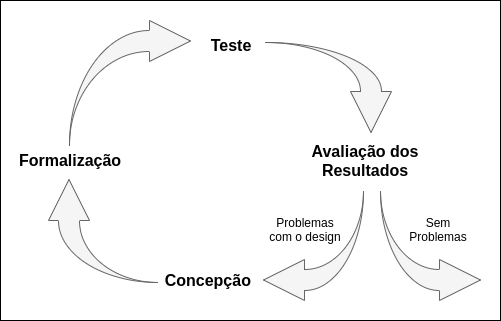
\includegraphics[keepaspectratio=true,scale=0.5]{figuras/playcentrtic_process.png}
	\caption{Diagrama de Processo Iterativo - adaptado de \citeonline{Fullerton_2008}}
	\label{Fig:playcentric_process.png}
\end{figure}

\subsection{Passo a Passo do Processo}

O \textit{Playcentric Design Process} é formado por alguns passos. Estes são etapas que servem para nortear o progresso do projeto de um jogo. Pode ser observado que apenas o passo \textit{Apresentação} não segue o fluxo iterativo além de ser opcional dentro do processo. Estes passos são ilustrados na Figura \ref{Fig:playcentric.png}. 

\begin{figure}[htbp]
	\centering
		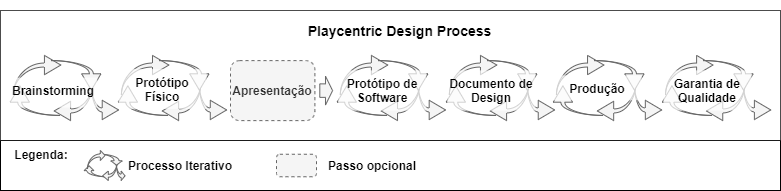
\includegraphics[keepaspectratio=true,scale=0.58]{figuras/playcentrtic.png}
	\caption{Fluxo Playcentric Design Process - Próprio Autor}
	\label{Fig:playcentric.png}
\end{figure}

Como pode ser visto na Figura \ref{Fig:playcentric.png}, o \textit{Playcentric Design Process} possui sete passos principais. Estes passos estão descritos a seguir e junto a eles estão inseridas algumas diretrizes da Engenharia de Software:

\begin{enumerate}
    \item \textbf{Brainstorming:} Segundo \cite[p. 155]{barbosa_silva} o brainstorming é uma técnica que fornece, de uma forma bastante livre, um conjunto de informações e opiniões sobre o tema e seus elementos que envolvem um projeto. % IHC pg 155
    Este é o pontapé inicial onde são concebidas as primeiras ideias ou sistemas de mecânica de jogo que poderão alcançar uma determinada meta de experiência do jogador. Essas ideias e sistemas são descritos brevemente e documentados. Por fim, estes conceitos são testados com jogadores em potencial \cite[p. 15]{Fullerton_2008}. % Playcentric pg 15
    Aqui neste passo é iniciada a tarefa de elaboração dos requisitos elicitados, onde as informações obtidas no levantamento de requisitos são refinadas, cujo nível de abstração já demonstra o comportamento do software \cite[p. 128]{Pressman_2000}.
   
    \item \textbf{Protótipo Físico:} o objetivo é desenvolver um projeto e revisão de alto nível \cite{Pressman_2000}, no qual o processo se baseia basicamente na técnica de prototipagem física, que fica a critério do designer qual o modelo será usado \cite{Fullerton_2008}. Segundo \citeonline{Fullerton_2008} o protótipo pode ser feito com papel, fichas, papelão, maquetes, figuras de plástico etc. O ponto chave do uso dessa técnica é a praticidade de se elaborar e fazer alterações, a interação que há com o jogador e o foco da equipe de design permanecer em validar conceitos sem a preocupação com o desenvolvimento do código do jogo \cite{Fullerton_2008}. 
    Outro ponto chave é que ele deve ser criado artesanalmente a partir dos conceitos elaborado e validados no passo anterior, de forma que possa ser "jogado". Ele então é testado e os resultados que demonstrarem uma jogabilidade funcional que atinge as metas de experiência do jogador devem ser descritas e documentadas \cite{Fullerton_2008}. % Playcentric pg 15; ES pg 74 %trazer referência técnica sobre prototipação de papel

    \item \textbf{Apresentação:} Este é um passo opcional em que o projeto é demonstrado às partes interessadas que podem financiar o desenvolvimento do jogo. Porém mesmo que não haja um necessidade de financiamento, o exercício de criar um apresentação completa é uma boa maneira de receber \textit{feedback} \cite{Fullerton_2008}. No caso, a apresentação pode ser representada pela defesa do trabalho, mediante a banca examinadora, que são algumas das partes interessadas % Playcentric pg 15

    \item \textbf{Protótipo de Software:} A partir dos modelos de protótipo físico elaborados e validados é possível começar a criação dos modelos de protótipos de software. Neste passo ainda deve se pensar em economia de tempo e não detalhar muito alguns aspectos, apenas o necessário para o teste. Seguindo o fluxo iterativo, agora o protótipo é testado e caso demonstre uma jogabilidade funcional que atinja as metas de experiência do jogador o processo segue para o próximo passo \cite{Fullerton_2008}. % Playcentric pg 15
    % Falar do modelo evolutivo de protótipo e sobre protótipo de alta fidelidade

    \item \textbf{Documento de Design:} Neste ponto são especificadas todas as ideias concebidas, prototipadas, testadas, validadas e já brevemente documentadas no \textit{Game Design Document} (GDD) \cite{Fullerton_2008}. Outro documento que auxilia na especificação do projeto é o \textit{Technical Design Document} (TDD), que trata não apenas do que precisa ser criado, mas também como será implementado \cite{Bethke_2003}. \citeauthor{Pressman_2000} diz que exitem várias formas de se especificar um sistema, porém o artefato deve ter um caráter flexível. Estes documentos de design não necessitam ser rigorosamente escritos inicialmente, logo após um primeiro rascunho completo já estar pronto inicia-se a fase de produção \cite{Fullerton_2008}. % Playcentric pg 15; ES pg 129


    \item \textbf{Produção:} Segundo \citeonline{Pressman_2000} o projeto deve ser refinado e revisado antes de dar o próximo passo, que é a implementação do código. Depois de todos esses passos de planejamento estarem bem fundamentados se inicia a criação da arte e da programação real do jogo. Para isso é feita a configuração do ambiente de desenvolvimento e é seguido algumas práticas metodológicas para a implementação do software. Paralelo a isso continua-se o processo iterativo de teste, avaliação e melhoria e a medida que isso for acontecendo os artefatos de design vão sendo refinados \cite{Pressman_2000, Fullerton_2008}. 
    
    
    \item \textbf{Garantia da Qualidade:} Neste último passo o projeto deve estar pronto para o teste de qualidade, já com uma jogabilidade bem sólida. Aqui é momento em que o jogo é trabalhado para ser acessível a todo o público-alvo \cite{Fullerton_2008}. % Playcentric pg 18
    
\end{enumerate}

Em seguida temos o capítulo que trata do referencial teórico. Esta parte do trabalho já é reflexo do resultado da primeira etapa do processo metodológico, que contempla a revisão da literatura.

% Trazer uma sessão falando das práticas ágeis adotadas?

% - Elaboração
%   - Elicitação e Análise dos Requisitos(questionário; brainstorm; Persona; Introspecção, base científica; RF e RFN(UX); backlog; priorização; cronograma do TCC2)
%   - Prototipação
%   - Ideação do Jogo(GDD)
%   - Aspectos técnicos do jogo(TDD)[Modelagem dos dados; Design da Arquitetura; Análise e Validação]


% TCC 2
%   - Pesquisa Científica:
%      - Apresentação dos Resultados
%      - Considerações Finais e Sugestão de Trabalhos Futuros
%   - Desenvolvimento de Software
%      - Gerência e Configuração do Ambiente (qualidade de escrita de código, bibliotecas, dependências, ferramentas, testes)
%      - Implementação 
%      - Testes 
%   - Continuidade do Projeto
%    - Elaborar Artefatos
%      - Artefatos de Design
%      - Artefatos Técnicos
